\chapter{Related Work}

With science and technology progressing rapidly, there is a good chance of availability of already implemented solution for a given problem identified in a target system. This chapter highlights the existing systems in place which provide solutions designed to achieve similar goals to the thesis under discussion and comparison to how the solution presented in the current document differs from them. This chapter is divided into two sections with the first section briefly describes the existing distributed systems which can be used for cluster computing followed by the second section focusing the use of distributed systems in the field of 3D printing.

\section{Introduction to distributed systems and its types}
A distributed system consists of autonomous systems (AS) connected through network which interact (if necessary) through message passing and most importantly give the user an illusion of being single large system \cite{DCE}. The main goal of distributed system is to connect the users and the available infrastructure i.e. IT resources, in a transparent, open, cost-effective, reliable, scalable way. Transparency in distributed computing environment (DCE) means that the user is unaware of the underlying system complexities in terms of location of the AS, heterogeneity of the system hardware, concurrency and replication of the AS mainly to provide reliability and fault tolerance. Transparency property of the distributed systems makes it appear as a single system dedicated to perform some tasks to the user \cite{DSBook}. Scalability refers to the property by which the number of AS in the DCE can be increased (scaled in) or decreased (scaled out) so as to provide best suited infrastructure to handle the fluctuating load (i.e. the amount of work to be done). The shared resources of the distributed system can be broadly classified as physical resources and virtual resources. The Figure\ref{fig:TypesOfResourceSharing} details the resources included in the two categorizes. 

\begin{figure}[ht!]
\centering
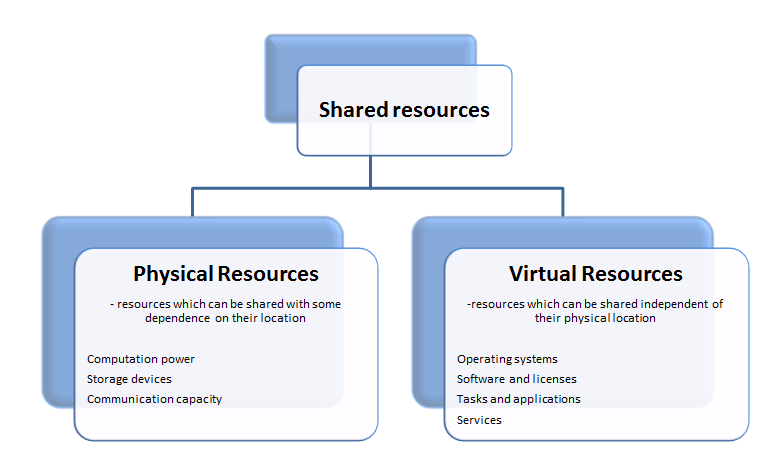
\includegraphics[scale=0.6]{TypesOfResourceSharing.PNG}
\caption{Distributed System Shared Resource Classification}
\label{fig:TypesOfResourceSharing}
\end{figure}
  
Distributed Computing is a vast domain which consists of various different types of computing environments like utility computing (grid computing and cloud computing), cluster computing, and peer-to-peer computing (Figure \ref{fig:DistributedComputingEnv}) which are described briefly as follows.

\begin{figure}[ht!]
\centering
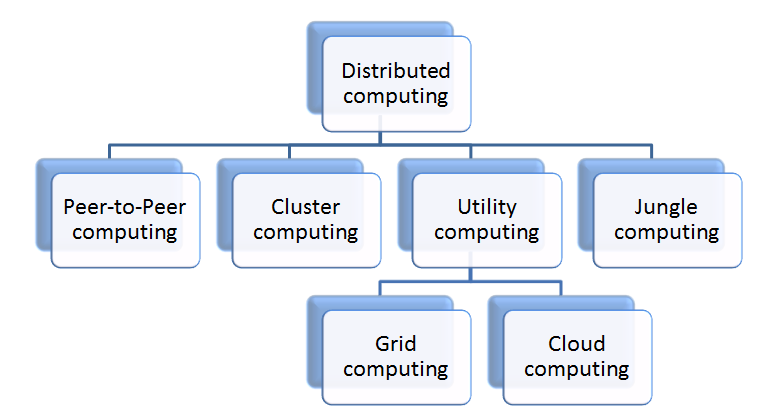
\includegraphics[scale=0.6]{DistributedComputingEnv.PNG}
\caption{Distributed Computing Environment}
\label{fig:DistributedComputingEnv}
\end{figure}

\begin{itemize}
\item \textbf{Peer-to-Peer computing}- Each node in the DCE acts as both client and server, providing as well as consuming part of the system resources. Peers are machines simply connected to the internet where in each peer can freely join and leave the DCE without affecting the whole system making the system self-organizing  and also implying no particular role (either master or slave) for a peer (Figure \ref{fig:P2P}).

\begin{figure}[ht!]
\centering
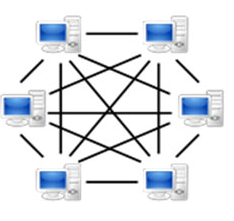
\includegraphics[scale=0.6]{P2P.PNG}
\caption{Peer-to-Peer system}
\label{fig:P2P}
\end{figure}

\item \textbf{Utility computing}- Utility computing is based on a model for service provisioning, which allows the users (consumers) to pay the providers for using the service only when they need to. It emphasizes on a business model, by which service providers make available the requested/paid resources to the costumers. All grid/cloud platforms are regarded as utility service providers. Grid computing enables coordinated resource sharing and problem solving in dynamic, multi-institutional virtual organizations where as cloud computing is a computing paradigm that involves outsourcing of computing resources with the capabilities of  replaceable resources and scalability i.e on-demand provisioning with little or no up-front IT infrastructure investment costs. Cloud computing offers its benefits through three types of delivery models namely- infrastructure-as-a-service (IaaS), platform-as-a-service(PaaS) and software-as-a-Service (SaaS) 

\item \textbf{Cluster Computing}- A cluster is a set of stand-alone computers and a network interconnecting them. The computers of the cluster work cooperatively together as a single integrated computing resource. A cluster is local if all of its component subsystems are supervised within a single administrative domain, usually residing in a single room and managed as a single computer system. The components of a cluster are connected to each other through fast local area networks. 

As mentioned in the brief description of different distributed systems, each node is similar to the other in a peer-to-peer system and it can join/leave the distributed system without affecting the user. As the requirement of the thesis design needed designated roles for the nodes, a peer to peer system does not fulfill the requirement of specific node roles in distributed system. A Peer-to-Peer system mostly uses internet to maintain connectivity amongst the peers. The distributed system to be used in the thesis has nodes which were connected through the enterprise network and it was not possible for a node outside the institution to join the system, which makes peer to peer system not an ideal choice. Grid computing essentially has systems which are offered by multiple institutions as resources, which dedicated to perform part of computation required for solving huge problems. The institutions which offer their systems form a virtual organization and only these institutions have shared access rights on the resources \cite{DSBook}. The distributed system in demand for the thesis is dedicated to be used for a specific enterprise and other institutions not part of the same network cannot contribute computes nodes. This makes grid computing not suitable as a distributed system for the thesis under discussion. 


\subsection{Use of Distributed Computing in fields involving large computations}

Distributed systems offer various advantages like computational speed-up, robustness through duplication of the resources, cheaper and scalable infrastructure etc. 
Using distributed systems allows to overcome the limitation of resources for solving problems with large computation, making it possible to get correct results within in a shorter span of time. The various domains where distributed computing has been used involves astronomy: for example Cosmology@Home is a project started to design models which describe the universe \cite{coshome}, data analysis and machine learning: the DistributedDataMining project involved data analysis for stock market prediction and analysis of medical information \cite{DisDataMin}, molecular biology: RNA world distributed system uses bio-informatics software to study the structure of RNA \cite{rnaworld}, climate study projects started in Oxford University use distributed system to study the climate changes which help to draw models for more accurate climate predictions \cite{ClimaProj}, etc. \newline

  


\section{Existing solutions for 3D Printing}

As described in the Introduction, 3D Printing is one of the upcoming additive manufacturing process and a favorite research topic. There are various solutions available in the market for varying kinds of requirements in terms of material, appearances, cost etc. Out of the many interesting solutions available, there are three solutions which are most relevant with respect to the current thesis topic as they use distributed system as an integral part of their solution. {\lq}\textbf{3dPrinterOS}{\rq} is a cloud-based management software for 3D printers which provides tools for making 3D printing user-friendly \cite{3dprinteros}. The user can connect the local 3D printer to the internet using the software provided by 3DPrinterOS thereby allowing the cloud-based software to drive the connected printer. It allows three input file formats (obj, amf and STL). The management software provides a tool to perform orientation of the print object on the print bed and to scale the size of the object as well as the slicer to perform slicing by allowing the user to set the slice thickness. The 3dPrinterOS software can be used only for the printers which are supported by it and does not act as a universal printer driver. The software allows to drive the connected printer but does not provide a way to generate output which can be then used to control the printer i.e. in our case bitmaps or STL output. During installation of the software to connect the local printer to the cloud, there are numerous device drivers which are installed on the client machine which might not always be ideal as there could be various trust issues associated with installation unknown device drivers from random sources. \newline

{\lq}\textbf{3DHubs}{\rq} is an online services which allows the user to provide digital input of the print object, select the material to be used to print the input and last but not the least select the print lab (where the object is printed locally and shipped to the user) by comparing the prices for printing the object \cite{3dhub}. It is a commercial solution to enable 3D Printing as a service where in the user does not need to own a 3D printer. It provides easy access to different kinds of material as well as helps to avoid setting up the required infrastructure to make use of the 3D Printing technology. It is quite beneficial and cheaper for users who do not print quite often but might not be an ideal solution for frequently printing customers. To use the solution the 3d model is uploaded to the server, which might not be desirable for companies where the design needs to be highly-protected. Also, there are no additional tools to provide dimensions if the digital input needs to be scaled up or down. \newline     

The {\lq}\textbf{Collaborative Cloud Printing Service}{\rq} is a cloud-based service for utilization of the 3D Printing resource developed by Institute of Computer-aided Product Development Systems at University of Stuttgart \cite{Baumann2016}. The solution provided is within the academic context and not a commercial solution. The focus of the project was to facilitate sharing of 3D Printing resources, provide platform for developing or extending and testing BPMS (Business Process Management Systems). The underlying distributed system used is the internet where as the approach in the current thesis is to use the enterprise network and computers within the network as distributed system which would be more desirable for companies who have privacy of their print models as the primary concern. The output for the cloud service under discussion is a printed object where as for the distributed cuttlefish the output is not necessarily a 3D printed object.  

